\section{Initialisierung des Server}
\section{Initialisierung der Datenbank }
\section{Initialisierung der Landingpage [L]}
\setauthor{Litzlbauer Lorenz}
Der erste Entwicklungsschritt für die vollständige Single-Page-Application beginnt mit der Initialisierung der Landingpage. Die Landingpage ist die Startseite der Webseite. Es ist das Erste, was der*die neue Nutzer*in sieht. Daher muss die Webseite alle benötigten Informationen über die Funktionen der Applikation verständlich erkennbar machen.

\subsection{Aufsetzen der Landingpage [L]}
\setauthor{Litzlbauer Lorenz}
Die Entwicklung startete damit, dass die benötigten Technologien Angular, AngularThree, AngularMaterials und Bootstrap heruntergeladen werden mussten.

Dafür wurde der \emph{npm} Node-Package-Manager verwendet.


\subsubsection{Vorbereitung}
Erstmal musste NodeJs installiert werden. Dafür wird aber zuvor noch NodeJs benötigt. NodeJs ist eine JavaScript Laufzeitumgebung. NodeJs kann von der eigenen Webseite nodejs.org mit dem Installer für alle Betriebssysteme installiert werden. Im Projekt wurde sich für eine LTS - Version(long term support) entschieden, weil diese am längsten von den Entwicklern am längsten unterstützt werden und dadurch beständiger sind. Während dem Installationsprozess von NodeJs kann durch eine Auswahl auch NPM installiert werden. 

\paragraph{npm - Node Package Manager}
Der Node Package Manager ist ein Softwareverwaltungstool zum Downloaden, Aktualisieren, Veröffentlichen und Verwalten von OpenSource-Programmen in der NodeJs-Umgebung. \cite{whatNpm} \cite{AboutNpm}

\subsubsection{Angular installieren}
Angular hat ein eigenes Tool, die Angular CLI (Command Line Interface), um Projekte zu erstellen, zu bearbeiten, Komponenten, Services und vordefinierte Codemodule hinzuzufügen und das Projekt zu bauen.

\begin{lstlisting}[caption={{Terminalm - Angular aufsetzen, Installation der CLI, Configuration eines neuen Projektes, Starten des Projektes}},language=bash]
npm install -g @angular/cli 
ng new Gallery
? Would you like to add Angular routing? Yes
? Which stylesheet format would you like to use? SCSS   [ https://sass-lang.com/documentation/syntax#scss ]
cd Gallery
ng serve -o
\end{lstlisting}

In der ersten Codezeile wird das Angular-CLI-Tool global von NPM installiert.
Danach wird mit dem Befehl ng new mit dem CLI-Tool ein neues Angular Projekt erstellt. Danach wird es mehrere Konfigurationsauswahlmöglichkeiten geben. Für dieses Projekt wurden Routing aktiviert und  als Stylesheet-Formatierung Scss ausgewählt. Danach wurde in das (Projekt-) Verzeichnis Gallery gewechselt und dort mit dem Befehl serve der ein Webpack-Server gestartet, welcher den vorgenerierten Code von dem neu erstellen Angular-Projekt zeigt (siehe in Abbildung \ref{fig:impl:angular-starting-page}). 

\begin{figure}[h t]
    \centering
    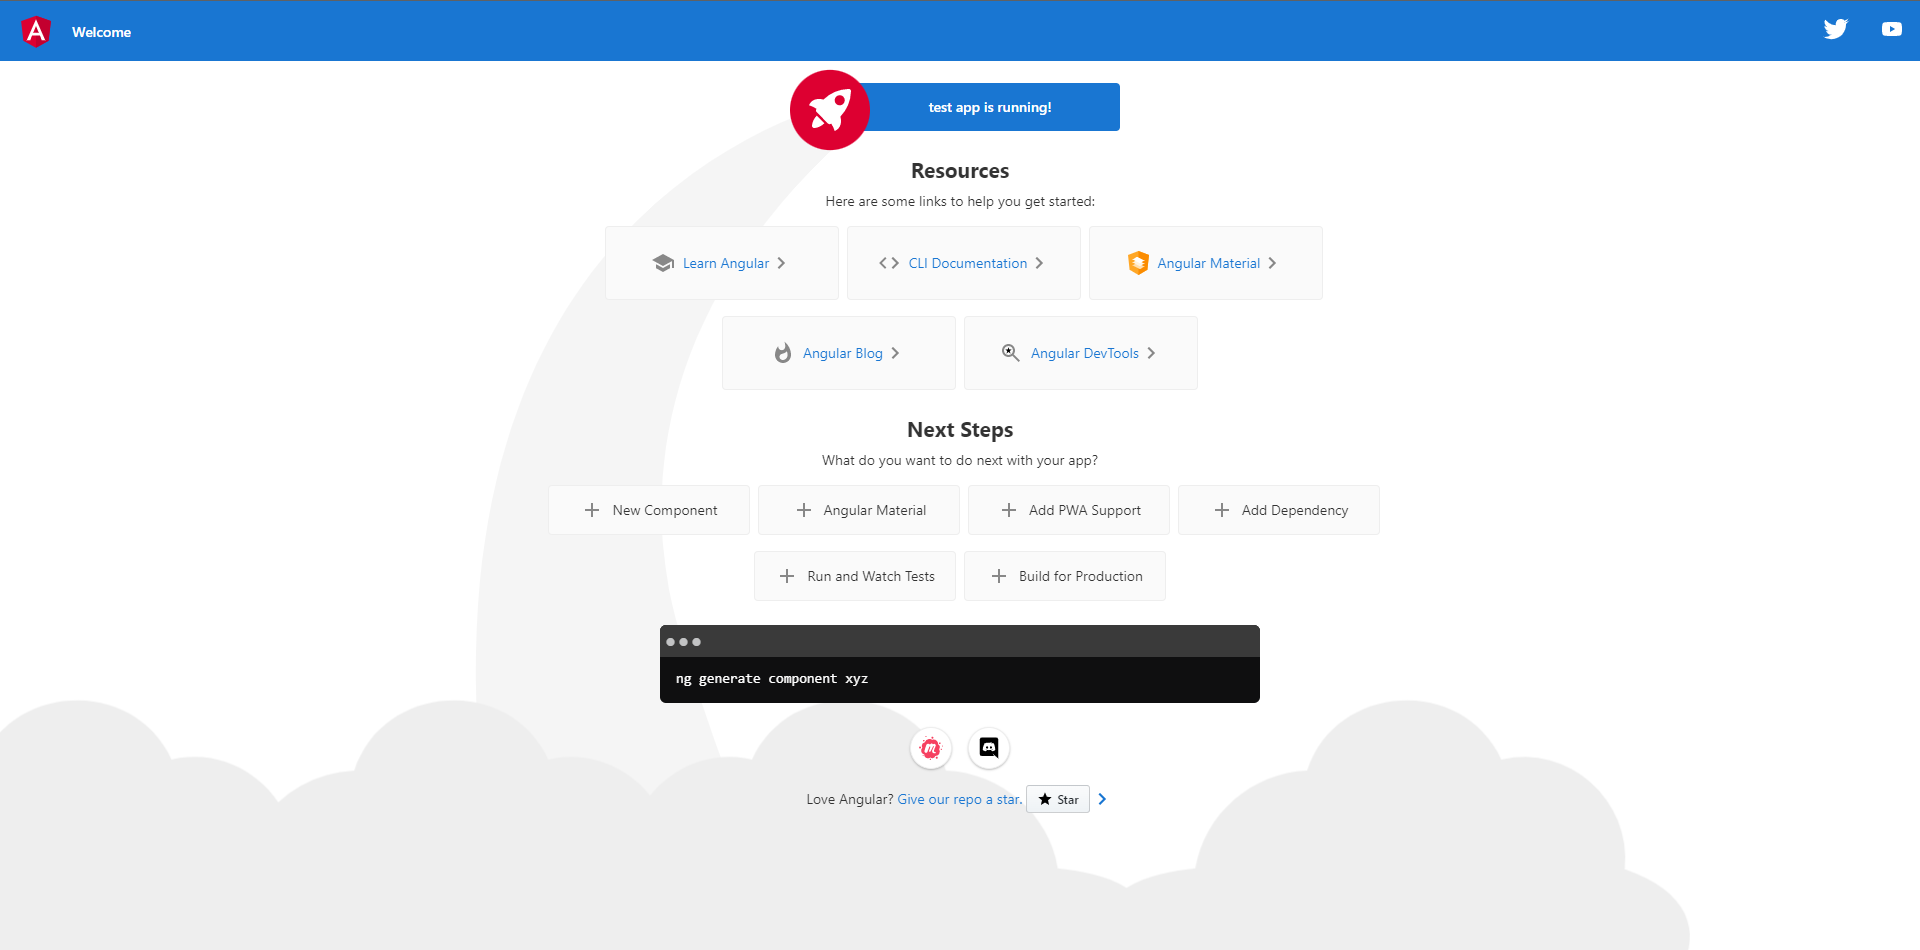
\includegraphics[scale=0.25]{pics/AngularStartingPage.png}
    \caption{Angular: Automatisch generierte Start-Webseite}
    \label{fig:impl:angular-starting-page}
\end{figure}

\paragraph{Globale oder Lokale Module}
Bei einer lokalen Installation werden die installierten Module in einem node-module Computerordner lokal im Projekt abgespeichert, während alle globalen Installationen in einem einzigen Computerordner, abhängig vom Computersystem gespeichert werden.
Generell kann man bei NPM-Module zwischen lokalen und globalen Installationen unterscheiden. In der Regel ist eine lokale Installation besser, denn referenzieren mehrere Projekte auf ein globales Modul, kann es dazu kommen, dass bei einer Aktualisierung des globalen Modules verschiedene Projekte, sei es wegen veralteten Funktionen oder neuer Logik, darauf anders reagieren und es zu Problemen bei diesen Projekten kommt.
Die Ausnahme von dieser Regel sind bei CLI-Modulen, diese könnten auch lokal installiert werden und mit dem Befehl npx ausgeführt werden, aber es macht mehr Sinn global, da nichts im Projekt darauf referenzieren muss.
\cite{npmlocalorglobal}

\subsubsection{Installation der UI-Framework}

Nach der Installation von Angular wurden die UI-Frameworks installiert. Angular Material konnte mithilfe des Befehls  \ref{lst:impl:installationAngularMaterials} mittels der Angular CLI in das Angularprojekt eingebunden werden.

\begin{lstlisting}[caption={{Terminal - Angular Material Installation}},language=bash,label=lst:impl:installationAngularMaterials]
    ng add @angular/material
\end{lstlisting}

Bootstrap konnte mithilfe des Befehls \ref{lst:impl:installationBootstrap} und von NPM installiert werden. Bootstrap wurde zwar dem Projekt hinzugefügt, Angular weiß aber davon noch nichts. Deswegen musste in der Anuglar-Konfigurationsdatei \emph{angular.json} die Bootstrap Scss-Liberay eingebunden werden. Das wird in diesem Code \ref{lst:impl:BootstraptConfig} veranschaulicht. 

\begin{lstlisting}[caption={{Terminal - Bootstrap Installation}},language=bash,label=lst:impl:installationBootstrap]
    npm i bootstrap
\end{lstlisting}

\begin{lstlisting}[caption={{angular.json - Bootstrap Angular Verknüpfung}},label=lst:impl:BootstraptConfig]
    {
        ...,
        "projects": {
            "Gallery": {
                ...,
                "architect": {
                    "build": {
                        ...,
                        "options": {
                            ...,
                            "styles": [
                                ...,
                                "node_modules/bootstrap/scss/bootstrap.scss"
                            ]
                        }
                    }
                }
            }
        },
        ...
    }
    
\end{lstlisting}


\subsubsection{Installation von Three Js}
Nach der Installation der UI-Libraries wurde ThreeJs installiert und in das Angular-Projekt eingebunden. 

TODO: Lorenz ThreeJs Einbindung beschreiben


